\documentclass[master]{NTHUthesis}
\usepackage[utf8]{inputenc}
\usepackage{subcaption}
\usepackage{amsmath}
\usepackage{amssymb}
\usepackage{booktabs}
\usepackage{graphicx} % Required for \resizebox
\usepackage{tabularx}
\usepackage{rotating}
\usepackage{makecell}
\usepackage{placeins}

%%% Customization  %%%
\usepackage{zhlipsum, lipsum}   % dummy text
\usepackage{graphicx}           % figures
\usepackage{booktabs}           % tables
\usepackage[ruled]{algorithm2e} % algorithms, list of algorithms
\usepackage{cite}               % bibliography
% \usepackage[numbers]{natbib}
\usepackage[authoryear]{natbib}

%%% Necessary %%%
\titleZH{論文名稱}
\titleEN{Thesis Title}

\instituteZH{資訊工程學系}
\studentID{112062000}
\studentZH{你的名字}
\studentEN{English Name}
\advisorZH{郭柏志}
\advisorEN{Po-Chih Kuo}
\yearZH{114} % 口試的年份
\monthZH{6} % 口試的月份

\begin{document}

\makecover

\pagenumbering{Roman}

%%% Necessary %%%
\begin{abstractZH}
% \zhlipsum[1-2]
中文摘要

關鍵詞:5~7 關鍵字。

\end{abstractZH}


%%% Necessary %%%
\begin{abstractEN}
% \lipsum[1-2]
This is your Abstract.

Keywords: 5~7 keywords.
\end{abstractEN}


%%% Optional %%%
\begin{acknowledgementsZH}
% \zhlipsum[1-2]
% Optional
\end{acknowledgementsZH}

%%% Optional %%%
% \begin{acknowledgementsEN}
% % \lipsum[1-2]
% % Optional
% \end{acknowledgementsEN}

%%% Necessary %%%
\maketoc

%%% Optional %%%
% \phantomsection
% \listofalgorithms
% \addcontentsline{toc}{chapter}{List of Algorithms}
% \clearpage

\pagenumbering{arabic}


\chapter{Introduction}
% \lipsum[1-3]
\section{Clinical Background}
\subsection{Risk of Prolonged Ventilation in ICU}
Mechanical ventilation is a critical life-support intervention in intensive care units for patients with respiratory failure \citep{ref02, ref01}. 

\subsection{Overview of the Traditional RL Framework}
In an RL framework shown in figure~\ref{fig:RL_framework}, an \emph{agent} interacts with an \emph{environment} to learn an optimal policy.

\begin{figure}[htbp]
  \centering
  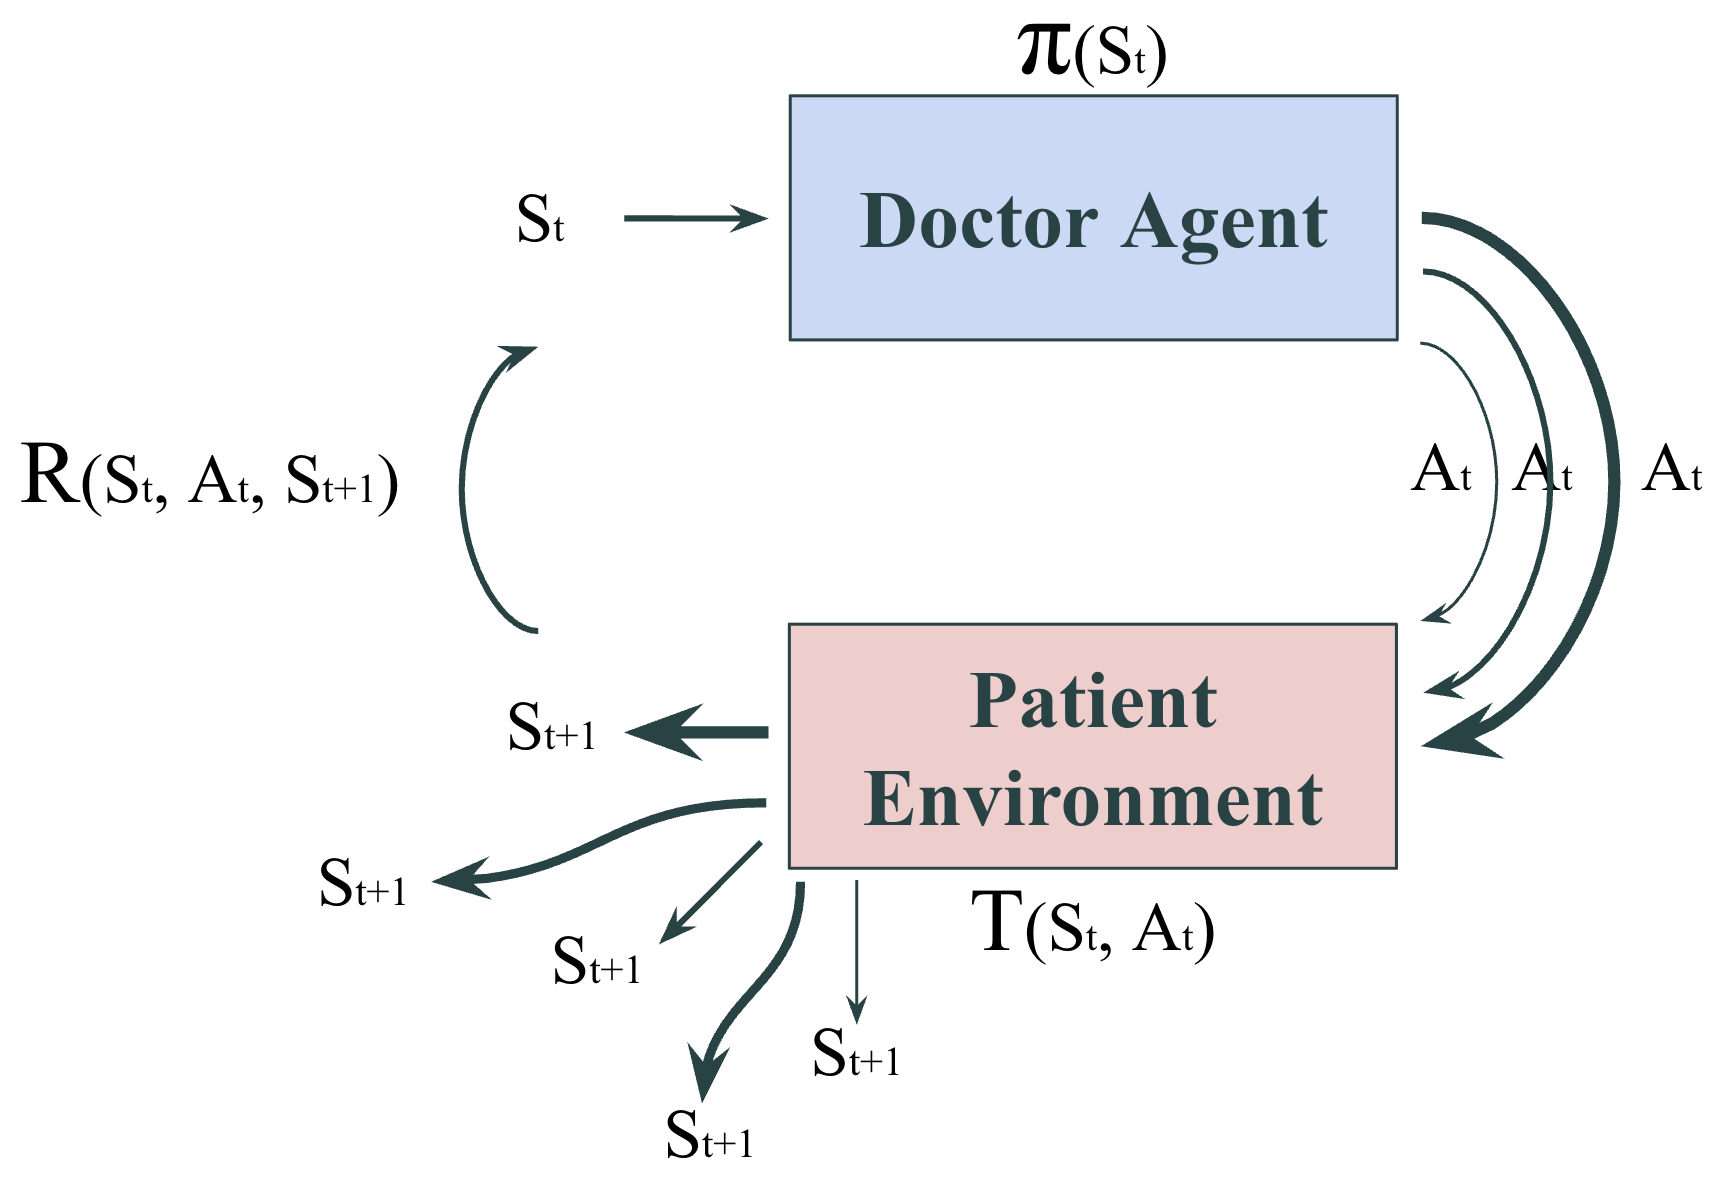
\includegraphics[width=0.7\textwidth]{figures/RL_framework.png}
  \caption{RL Framework with Stochastic Transitions and Variability in Physician Ventilator Strategies.}
  \label{fig:RL_framework}
\end{figure}
% \begin{table}[t]
%     \centering
%     \begin{tabular}{ c | c c }
%     \toprule
%      cell1 & cell2 & cell3 \\
%     \midrule
%      cell4 & cell5 & cell6 \\  
%      cell7 & cell8 & cell9 \\
%     \bottomrule
%     \end{tabular}
%     \caption{An example table}
%     \label{tab:my_label}
% \end{table}

\chapter{Related Works}
% \lipsum[1-3]
% This is Related Works.
% \begin{figure}
%     \centering
%     \includegraphics[width=.6\linewidth]{example-image-a}
%     \caption{An example figure.}
%     \label{fig:example-a}
% \end{figure}

% \section{Section Title}
% \lipsum[4-5]

% \subsection{Subsection Title}
% \lipsum[6]

\chapter{Methodology}
% \lipsum[1-3]
% This is Methodology.

% \begin{algorithm}[t]
% \SetAlgoLined
% \KwResult{Write here the result }
%  initialization\;
%  \While{While condition}{
%   instructions\;
%   \eIf{condition}{
%    instructions1\;
%    instructions2\;
%    }{
%    instructions3\;
%   }
%  }
%  \caption{How to write algorithms}
% \end{algorithm}

\chapter{Experiments}
% This is your Experiments.

\chapter{Results}
% This is Results.


% Compact reward design table with highlighting for BCQ on train
\begin{table}[htbp]
\centering
\caption{Reward Design Comparison Across All Severity Categories for Training Set (BCQ).}
\small
\resizebox{\textwidth}{!}{%
\begin{tabular}{lccc|ccc|ccc|ccc|ccc}
\toprule
\textbf{Metric} & \multicolumn{3}{c}{\texttt{default}} & \multicolumn{3}{c}{\texttt{NoActPen}} & \multicolumn{3}{c}{\texttt{NoIntermRew}} & \multicolumn{3}{c}{\texttt{HighExtubRew}} & \multicolumn{3}{c}{\texttt{NoExtubRew}} \\
 & High & Med & Low & High & Med & Low & High & Med & Low & High & Med & Low & High & Med & Low \\
\midrule
Total Cumulative Reward & 6.64 & 8.55 & \textbf{9.44} & 6.59 & \textbf{8.67} & 9.15 & 6.68 & 8.61 & 9.06 & \textbf{7.01} & 8.42 & 9.27 & 6.99 & 8.48 & 9.24 \\
Extubation Meet Rate (\%) & 94.0 & \textbf{100.0} & \textbf{100.0} & 93.0 & \textbf{100.0} & \textbf{100.0} & 92.0 & \textbf{100.0} & \textbf{100.0} & \textbf{95.0} & \textbf{100.0} & \textbf{100.0} & \textbf{95.0} & 99.0 & \textbf{100.0} \\
Avg. Trajectory Length (hrs) & 16.72 & 14.5 & \textbf{12.39} & 16.11 & \textbf{14.27} & 12.79 & 15.58 & 15.52 & 13.6 & \textbf{15.41} & 16.43 & 13.51 & 19.8 & 16.5 & 13.23 \\
Avg. Time to Meet (hrs) & 17.53 & 14.5 & \textbf{12.39} & 17.0 & \textbf{14.27} & 12.79 & 16.57 & 15.52 & 13.6 & \textbf{15.99} & 16.43 & 13.51 & 20.63 & 16.63 & 13.23 \\
Action Diversity & 16 & 9 & 13 & 14 & 10 & 13 & 15 & \textbf{14} & \textbf{17} & 17 & 10 & 14 & \textbf{30} & \textbf{14} & 14 \\
Anomalous Actions (\%) & 6.0 & \textbf{0.0} & \textbf{0.0} & 7.0 & \textbf{0.0} & \textbf{0.0} & 8.0 & \textbf{0.0} & \textbf{0.0} & \textbf{5.0} & \textbf{0.0} & \textbf{0.0} & \textbf{5.0} & 1.0 & \textbf{0.0} \\
\bottomrule
\end{tabular}
}%
\label{tab:reward_design_comparison_highlighted_DiscreteBCQ_train}
\end{table}

\chapter{Discussion}
% This is your Discussion.

\chapter{Conclusion}
% This is your Conclusion.
% This is the demo of cite ref01~\cite{ref01}
% This is a dummy sentence~\cite{Alpher02}. This is a dummy sentence~\cite{Alpher03, Alpher02}~\cite{Alpher05}~\cite{Alpher06}~\cite{Alpher07}~\cite{Alpher08}~\cite{Alpher09}. This is a dummy sentence~\cite{Alpher04}. A dummy Text\footnote{A dummy footnote.}.

% \clearpage
% \chapter{Supplementary}
% \input{sections/supplementary}

% \bibliographystyle{plain}
\bibliographystyle{apalike}
\bibliography{references}

\end{document}
